\chapter{Multirate implementation}
The chapter will describe the three functions which is used in the multirate stages.
\begin{itemize}
\item void downFunc1(int16 dataIn);
\item int16 delayB1(int16 dataIn);
\item int16 upFunc1(int16 dataIn,int16 band);
\end{itemize}
Where downFunc1 is used to decimate and spectral subtract the input sample, delayB1 is used to delay a sample by x samples and upFunc1 is used interpolate the input sample (dataIn) and add the input sample (band) to the interpolated signal. In both downFunc1 and upFunc1 a filter function is used called FIR1 which runs a FIR filter on a data array, which also will be decribed in this chapter. 



\section{Decimation and spectral subtraction implementation}
The decimation block is described in \textbf{XX} and is seen on \autoref{fig:DownsamplingSimulationCopy}.
\begin{figure}[H]
    \centering
	\includegraphics[width=\textwidth, page=2]{Simulation}
    \caption{Decimation block diagram}
    \label{fig:DownsamplingSimulationCopy}
\end{figure}
The block contains different components which has to be implemented:
\begin{itemize}
\item Reading data in.
\item FIR filtering.
\item Spectral subtraction.
\item Downsampling and outputting. 
\end{itemize}




\section{Interpolation implementation}
The interpolation block is described in \textbf{XX} and is seen on \autoref{fig:upsamplingSimulationCopy}.
\begin{figure}[H]
    \centering
	\includegraphics[width=\textwidth, page=11]{Simulation}
    \caption{Interpolation block diagram}
    \label{fig:upsamplingSimulationCopy}
\end{figure}
The block contains different component which has to be implemented:
\begin{itemize}
\item Reading in data and upsampling.
\item FIR filtering
\item Spectral addition
\end{itemize}


\section{delay implemetation}
The delay block delays a sample x times this is done by implementing a circular buffer with a pointer. The flowchart seen on XX shows the flow of the algorithm.
\todo[inline]{FLOWCHART af delay funktion}
The function uses the following variables:
\begin{itemize}
\item XX
\end{itemize}


\section{FIR filter implementation}